\chapter{Background \& Related Work}\label{ch:background}

\section{The Semantic Gap}
One of the core insights of computer vision in general and content based image
retrieval in specific probably is that human perception is inseparably linked
to interpretation by the brain. As a human individual there is no way to
directly access visual information without them having been filtered and
weighted by one's personal experiences and cultural context. Therefore, when
people talk about visual similarity of images, it usually includes a large
degree of semantic similarity unconciously added to the perception. The
difference between that mode of perception and the current algorithmic ways to
analyse visual data has been eloquently coined \emph{the semantic gap} by
\autocite{smeulders_content-based_2000}:

\begin{quote}
The semantic gap is the lack of coincidence between the information that one
can extract from the visual data and the interpretation that the same data have
for a user in a given situation.
\end{quote}

Having had that realisation can guide the decision of a researcher or designer
of such systems.

\section{The Sensory Gap}
In addition to the semantic ambiguity described above, another major obstacle
of computer vision impacts a CBIR system: \emph{the sensory gap}. This term has
also been coined by \autocite{smeulders_content-based_2000}, where it's defined
as follows:

\begin{quote}
The sensory gap is the gap between the object in the world and the information
in a (computational) description derived from a recording of that scene.
\end{quote}

That terse definition includes a multitude of conditions, that can affect an
image, which a CBIR system operates on:

\begin{description}
    \item[Illumination] The brightness or direction of the illumination can
        hide or accent edges and texture properties in the scene. Similarly,
        the color of the illumination influences the recorded color information
        in the image.
    \item[Resolution] The imaging resolution sets a lower limit on the size of
        features that can be correctly recognised by any algorithm. As in all
        signal processing applications, aliasing of high frequency components
        of the image can introduct further ambiguities.
        \autocite{shannon_communication_1998}
    \item[Occlusion] Depending on the viewpoint of the recording and the
        composition of the scene, distinguishing parts of depicted objects may
        be occluded by other objects or objects may be only partially inside
        the recorded image.
    \item[Perspective] An object's proportions can be distorted by the imaging
        perspective.
\end{description}

An ideal CBIR system would use feature extraction and comparison methods that
can account and correct for such conditions.

\section{Anatomy of a CBIR System}
\begin{figure}[h]
    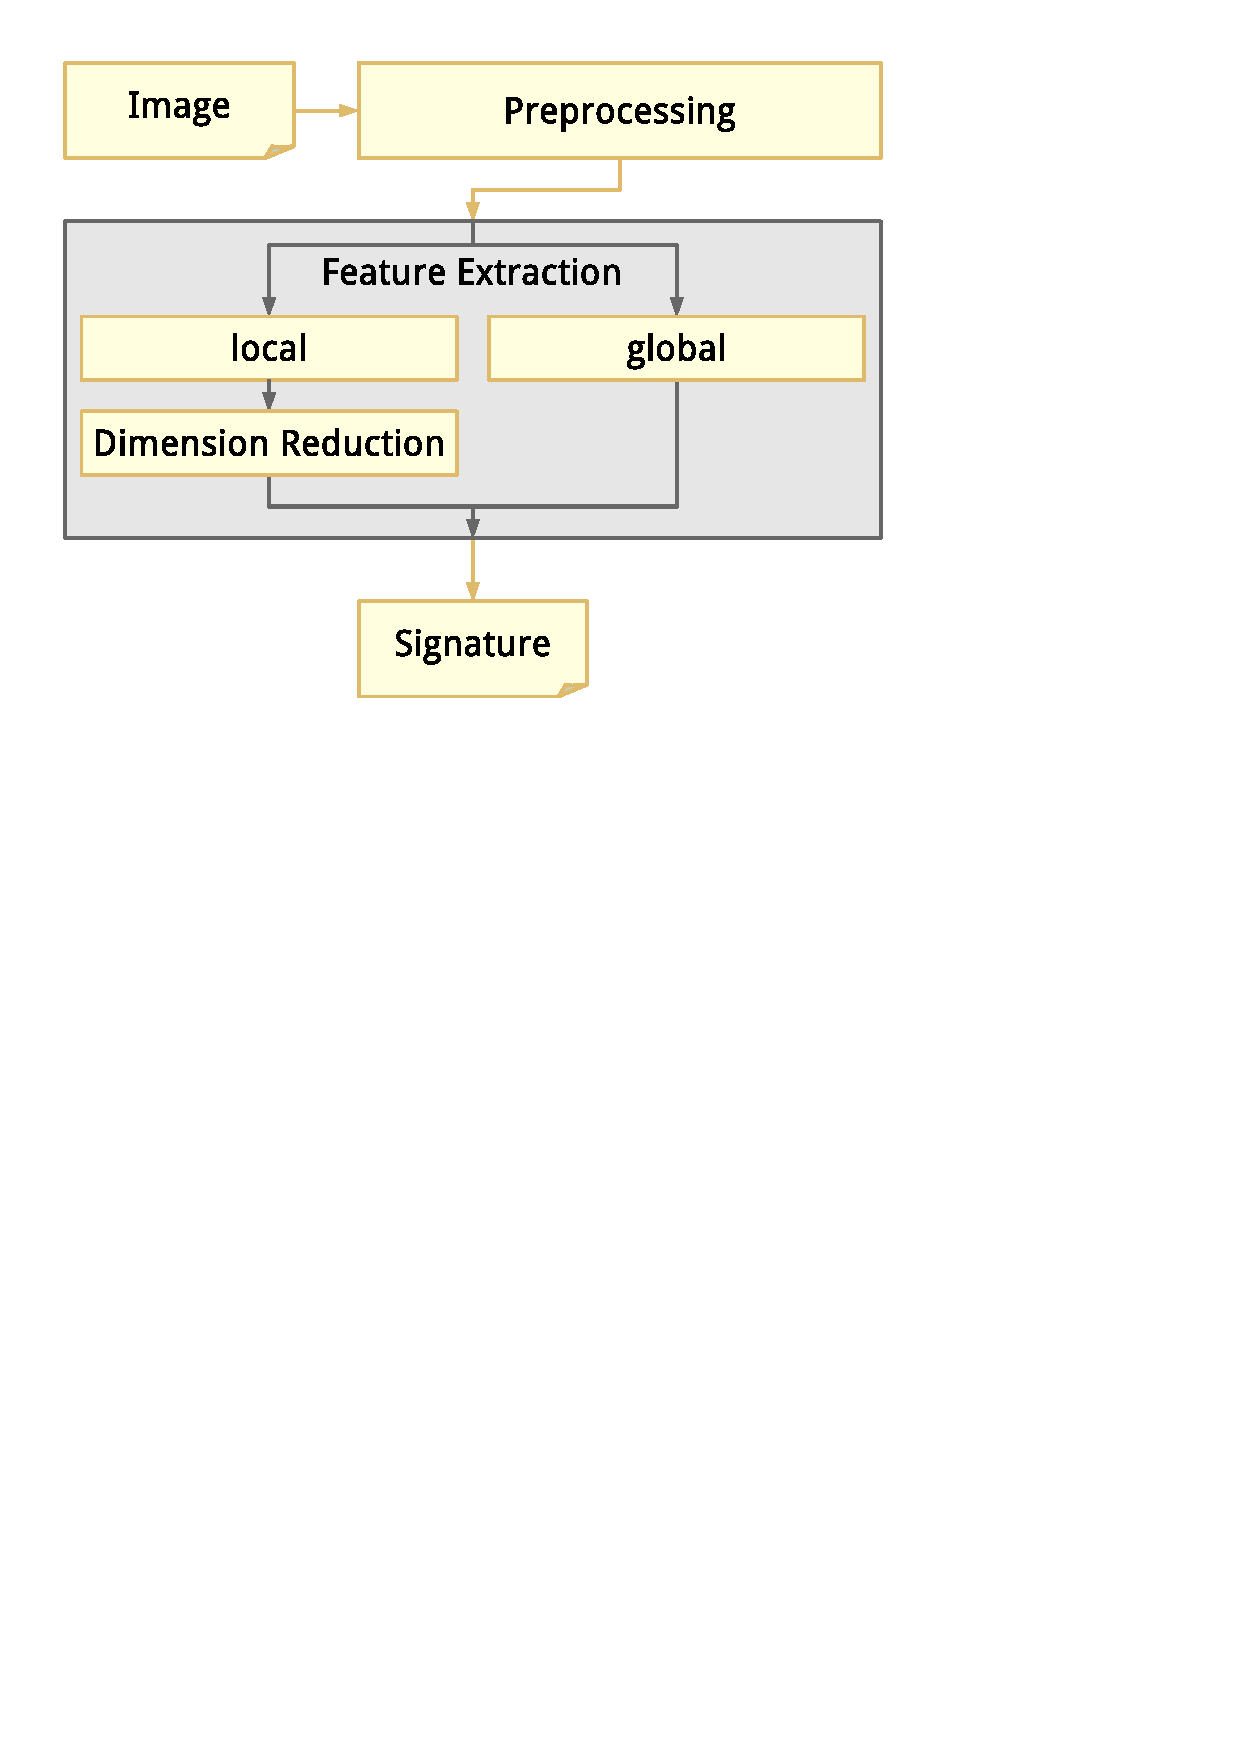
\includegraphics[width=0.8\textwidth]{cbir_anatomy}
\end{figure}
Illustration of basic structure of CBIR using local/global features.

Most approaches can be characterized by looking at three stages in their processing pipeline:

\begin{description}
    \item[Input format] The structure of the input data determines the amount of information available to the subsequent processing steps. Possible preprocessing steps include color space conversion, scaling and edge extraction.
    \item[Extracted features] Many algorithms produce a large number of coefficients that can be reduced to a set of feature coefficients using by techniques such as vector quantization or principal component analysis (PCA).
    \item[Distance metric] In order to rank the images according to similarity a metric is used to calculate the distance in feature space between two sets of feature coefficients. The selection of a metric is often closely coupled with the feature extraction algorithm.
\end{description}

\subsection{input format}
Complete vs incomplete sketches, intra-/cross-domain

\subsection{features}

\begin{itemize}
    \item bag of features from k-means clustered visual words [video google]
    \item histogram of oriented gradients [chalechale + refs]
\end{itemize}

\subsection{metric}

\begin{itemize}
    \item after ranking using euclidean distance, rank by spatial similarity [video google]
    \item Earth Mover's distance? [rubnerljcv00]
\end{itemize}
